\section{Rematching using quadrupole scans \textbf{Tobias}}

Uncertainties for the measurements
\begin{itemize}
\item Dispersion
\item Screen calibration
\item The fitting
\item The local model
\end{itemize}


\begin{figure}
\begin{center}
% 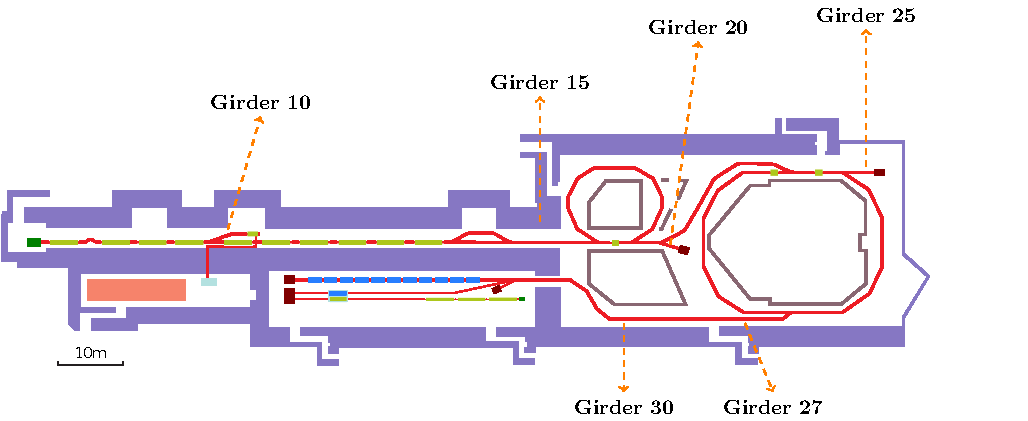
\includegraphics[width=1\linewidth,natwidth=493,natheight=202]{Screen_Layout.pdf}
 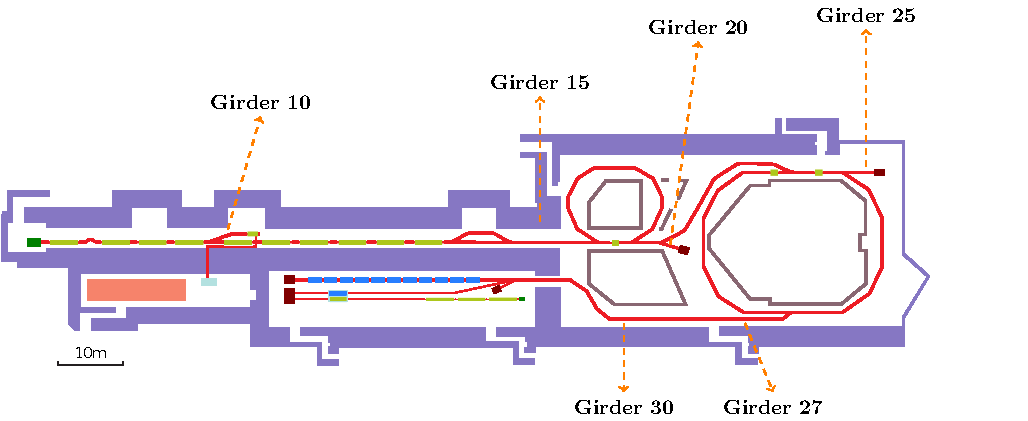
\includegraphics[width=1\linewidth]{Screen_Layout.pdf}
 \caption{The placements of the MTV screens used for measuring the beam parameters in CTF3. }
\label{fig:layout_screens}
\end{center}
\end{figure}

\subsection{Middle of the linac, Girder 10}
This screen has been used to optimize the emittance coming from the injector. 
This is done through adjusting the phases of the injector and by adjusting the strength of the solenoids. 
The other purposes has been to use this screen to rematch the optics functions. 
This is done through back propagating the parameters to girder 6 and then rematch. 
Attempts to re-match from girder 4 has also been done. 
A complication with this rematching is that the beam energy is not constant. 
The energy is measured in the spectrometer and than the energy is calculated at 
each location using the knowledge of the RF-power and the beam current. 

The first part of the emittance optimization is also done using this screen. 
It is important to control the orbit and the strength of the solenoids to get a low emittance. 


\todo{Example of a successful rematch and a possibly emittance step... }

\subsection{End of the Linac, Girder 15}

\todo{find a two different emittances but different range}

\subsection{Entrance of the Delay-Loop}
The optics function at the entrance of the delay-loop are important. 
This is because to have to have a beam with the same beam parameters coming out from 
the ring you need that the initial conditions are correct. 
This has been done through measuring in CTS back propagate the parameters to 
the end of the linac and do a re-match. This has in general been successful and 
an example is shown 
\todo{A good figure showing the success of the matching}%
\subsection{Limiting factors}
